\documentclass[11pt]{article}
\usepackage[UTF8]{ctex}
\usepackage[a4paper]{geometry}
\geometry{left=2.0cm,right=2.0cm,top=2.5cm,bottom=2.5cm}

\usepackage{caption}
\usepackage{paralist}
\usepackage{enumitem}
\setenumerate[1]{itemsep=0pt,partopsep=0pt,parsep=0pt,topsep=0pt}
\setitemize[1]{itemsep=0pt,partopsep=0pt,parsep=0pt,topsep=0pt}
\usepackage{comment}
\usepackage{booktabs}
\usepackage{graphicx}
\usepackage{float}
\usepackage{diagbox}
\usepackage{amsmath,amsfonts,graphicx,amssymb,bm,amsthm}
\usepackage{algorithm,algorithmicx}
% \usepackage[ruled, linesnumbered]{algorithm2e}
% \usepackage[linesnumbered]{algorithm2e}
\usepackage[noend]{algpseudocode}
\usepackage{fancyhdr}
\usepackage{tikz}
\usepackage{graphicx}
\usetikzlibrary{arrows,automata,positioning}
\usepackage{hyperref}
\usepackage{extarrows}
\usepackage{wrapfig}
% 这是一些字体选项
\usepackage{helvet}
% \usepackage{mathpazo}
\usepackage{fontspec}
% \setmainfont{Times New Roman}
% \setmainfont{Comic Sans MS} % 比较fancy的字体
% \setmainfont{Avenir}
% \setmainfont{Palatino}

\setlength{\headheight}{14pt}
\setlength{\parindent}{0 in}
\setlength{\parskip}{0.5 em}


\newtheorem{theorem}{Theorem}
\newtheorem{lemma}[theorem]{Lemma}
\newtheorem{proposition}[theorem]{Proposition}
\newtheorem{claim}[theorem]{Claim}
\newtheorem{corollary}[theorem]{Corollary}
\newtheorem{definition}[theorem]{Definition}
\newtheorem*{definition*}{Definition}

% \newenvironment{problem}[2][Problem]{\begin{trivlist}
% \item[\hskip \labelsep{\bfseries#1}\hskip\labelsep{\bfseries#2.}]}{\hfill$\blacktriangleleft$\end{trivlist}}
% 标题后强制换行
\newenvironment{problem}[2][Problem]{\begin{trivlist}
    \item[\hskip \labelsep{\bfseries#1}\hskip\labelsep{\bfseries#2.}]\mbox{}\newline}{\hfill$\blacktriangleleft$\end{trivlist}}
\newenvironment{answer}[1][Answer]{\begin{trivlist}
\item[\hskip \labelsep{\bfseries\itshape#1.}\hskip \labelsep]}{\hfill$\lhd$\end{trivlist}}

\DeclareMathOperator*{\minimize}{minimize}
\DeclareMathOperator*{\maximize}{maximize}
\newcommand\E{\mathbb{E}}
\newcommand\per{\mathrm{per}}
\renewcommand{\algorithmicrequire}{\textbf{Input:}}
\renewcommand{\algorithmicensure}{\textbf{Output:}}
\algrenewcommand{\algorithmiccomment}[1]{\hfill $//$ #1}
% chktex-file 44
% \renewcommand{\familydefault}{\sfdefault}

\RequirePackage{algorithm}

\makeatletter
\newenvironment{breakablealgorithm}
  {% \begin{breakablealgorithm}
    \begin{center}
      \refstepcounter{algorithm}% New algorithm
      \hrule height.8pt depth0pt \kern2pt% \@fs@pre for \@fs@ruled
      \parskip 0pt
      \renewcommand{\caption}[2][\relax]{% Make a new \caption
        {\raggedright\textbf{\fname@algorithm~\thealgorithm} ##2\par}%
        \ifx\relax##1\relax % #1 is \relax
          \addcontentsline{loa}{algorithm}{\protect\numberline{\thealgorithm}##2}%
        \else % #1 is not \relax
          \addcontentsline{loa}{algorithm}{\protect\numberline{\thealgorithm}##1}%
        \fi
        \kern2pt\hrule\kern2pt
     }
  }
  {% \end{breakablealgorithm}
     \kern2pt\hrule\relax% \@fs@post for \@fs@ruled
   \end{center}
  }
\makeatother

% set for automata
\tikzset{>=stealth',shorten >=1pt,auto,node distance=2cm, % Increase node distance to 4cm
                    thick,main node/.style={circle,draw,font=\sffamily\Large\bfseries}}


\title{Homework \#7}
\usetikzlibrary{positioning}

\begin{document}
\captionsetup[figure]{labelfont={bf},name={Fig.},labelsep=period}
\kaishu

\pagestyle{fancy}
\lhead{\CJKfamily{zhkai} Peking University}
\chead{}
\rhead{\CJKfamily{zhkai} Algorithm Design and Analysis (Honor Track)}

\begin{center}
    {\LARGE \bf Homework 7}\\
    {Name: 方嘉聪\ \  ID: 2200017849}            % Write down your name and ID here.
\end{center}

\begin{problem}{1. (Max Flow, Min Cut, and Duality)}
    In this exercise, we will demonstrate that LP duality can be used to show the max-flow min-cut theorem.

Consider the following instance of max flow:
\begin{figure}[h]
    \centering
    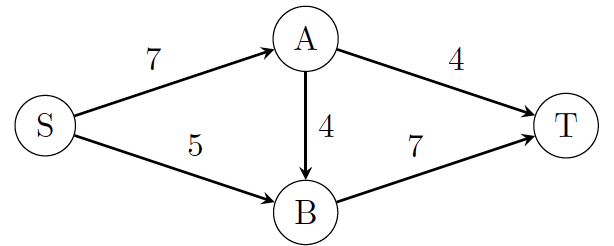
\includegraphics[width=0.4\textwidth]{figs/netflow1.png}
\end{figure}

Let $f_1$ be the flow pushed on the path $\{S,A,T\}$, $f_2$ be the flow pushed on the path $\{S,A,B,T\}$, and $f_3$ be the flow pushed on the path $\{S,B,T\}$. The following is an LP for max flow in terms of the variables $f_1, f_2, f_3$:
\begin{align*}
    \text{max } f_1+f_2+f_3 &\\
    f_1 + f_2 \leqslant 7 &  \text{\qquad (Constraint for $(S,A)$)}\\
    f_3 \leqslant 5 &   \text{\qquad (Constraint for $(S,B)$)}\\
    f_1 \leqslant 4 &   \text{\qquad (Constraint for $(A,T)$)}\\
    f_2 \leqslant 4 &   \text{\qquad (Constraint for $(A,B)$)}\\
    f_2 + f_3 \leqslant 7&  \text{\qquad (Constraint for $(B,T)$)}\\
    f_1, f_2, f_3 \geqslant 0&
\end{align*}
(a) Find the dual of this LP, where the variables in the dual are $x_e$ for each edge $e$ in the graph.

(b) Show that the dual of the LP for any max-flow problem is an LP for the corresponding min-cut problem.
\end{problem}
\begin{answer}
   (a) 把原问题的线性规划写成矩阵形式:
   \begin{align*}
    \maximize \quad&
    \begin{pmatrix} 
        1 & 1 & 1
    \end{pmatrix} \begin{pmatrix}
        f_1\\
        f_2\\
        f_3
    \end{pmatrix} 
    \\ \text{subject to} \quad &
    \begin{pmatrix}
        1 & 1 & 0 \\
        0 & 0 & 1 \\
        1 & 0 & 0 \\
        0 & 1 & 0 \\
        0 & 1 & 1 
    \end{pmatrix} \begin{pmatrix}
        f_1 \\
        f_2 \\
        f_3
    \end{pmatrix} \le \begin{pmatrix}
        7 \\
        5 \\
        4 \\
        4 \\
        7
    \end{pmatrix} \\
    & f_1, f_2, f_3 \ge 0
   \end{align*} 
    那么对偶问题为:
    \begin{align*}
        \minimize \quad&
        \begin{pmatrix}
            7 & 5 & 4 & 4 & 7
        \end{pmatrix} \begin{pmatrix}
            x_{(S,A)} \\
            x_{(S,B)} \\
            x_{(A,T)} \\
            x_{(A,B)} \\
            x_{(B,T)}
        \end{pmatrix} \\    
        \text{subject to} \quad
        & \begin{pmatrix}
            1 & 0 & 1 & 0 & 0 \\
            1 & 0 & 0 & 1 & 1 \\
            0 & 1 & 0 & 0 & 1
        \end{pmatrix} \begin{pmatrix}
            x_{(S,A)} \\
            x_{(S,B)} \\
            x_{(A,T)} \\
            x_{(A,B)} \\
            x_{(B,T)}
        \end{pmatrix} \ge \begin{pmatrix}
            1 \\
            1 \\
            1
        \end{pmatrix} \\
        & x_{(S,A)}, x_{(S,B)}, x_{(A,T)}, x_{(A,B)}, x_{(B,T)} \ge 0
    \end{align*}
    其中$x_e, \forall e \in E$表示边$e$是否在割集中(是为1, 否为0), 约束即为每条$s$-$t$路径至少有一条边在割中, 那么对偶问题是一个整数线性规划, 可以看出对偶问题是对应的最小割问题.

    (b) 考虑一个任意的有向图$G = (V,E)$, 源点$s$, 汇点$t$, 边容量$c(e)$. 设\[P = \{p \mid p \text{ is a simple path from $s$ to $t$}\}\] 注意到如果一个流有环, 那么去掉环不会使得流变差, 故我们这里只考虑简单路径. 那么类似第一问, 最大流问题的线性规划形式为($f_p$表示路径$p$的流):
    \begin{align*}
        \maximize \quad & \sum_{p \in P} f_p \\
        \text{subject to} \quad & \sum_{p \in P: (u,v) \in p} f_p \le c(u,v), \quad \forall (u,v) \in E \\
        & f_p \ge 0, \quad \forall p \in P 
    \end{align*}
    写成矩阵形式有(不妨设$|P| = m, |E| = n$):
    \begin{align*}
        \maximize \quad & \bm{1}^T \bm{f} \\
        \text{subject to} \quad & \bm{A} \bm{f} \le \bm{c} \\
        & \bm{f} \ge 0
    \end{align*}
    其中$\bm{f} = (f_i)_m, \bm{c} = (c_i)_n$, $\bm{A} = (A_{ij})_{n\times m}$, $A_{ij}$表示边$e_i$是否在路径$p_j$上. 那么对偶问题为
    \begin{align*}
        \minimize \quad & \bm{c}^T \bm{x} \\
        \text{subject to} \quad & \bm{A}^T \bm{x} \ge \bm{1} \\
        & \bm{x} \ge 0
    \end{align*}
    其中$\bm{x} = (x_i)_n$表示边$e_i$是否在割集中, 则最小割问题等价对偶的整数线性规划. 那么下面问题在于这一整数线性规划和原对偶线性规划的解是否相同.
    
    我们可以证明整数网络流问题的约束矩阵$\bm{A}$是一个全幺模矩阵(TUM)\footnote{这个证明太复杂, 引入了网络矩阵(Network Matrices)的概念, 我在网上找到了这个notes给出了详细证明 \url{https://webdocs.cs.ualberta.ca/~zacharyf/courses/combopt_2016/notes/lec16.pdf}}, 那么由课上提到的整数流定理\footnote{整数流定理: 如果网络流问题的流入、流出、边容量都是整数,目标函数也是线性函数,那么 对应的线性规划所有的基本可行解都是整数解. 一般的, 约束矩阵是TUM(Totally Unimodular Matrix)的线性规划存在整数最优解.}可知, 整数线性规划和原对偶线性规划的解是相同的. 证毕.
\end{answer}

\begin{problem}{2. (Network Flow with Vertex Capacities)}
    Let $G=(V,E)$ be a directed graph with a source vertex $s\in V$ and a sink vertex $t \in V$. Whereas the standard network flow problem involves capacities for edges, here we suppose instead that every vertex $v\in V$ has an integer capacity $c_v \geqslant 0$. A \textit{vertex-capacitated} flow in $G$ is a function $f: E \rightarrow [0,+\infty)$ such that
    \begin{itemize}
        \item (Capacity Constraint) For each vertex $v\in V$, we have
        $$
        \sum_{e\text{ into }v} f(e) \leqslant c_v \text{ and } \sum_{e\text{ out of }v} f(e) \leqslant c_v
        $$
        
        \item (Conservation Constraint) For each vertex $v\in V/\{s,t\}$, we have
        $$
        \sum_{e\text{ into }v} f(e) = \sum_{e\text{ out of }v} f(e)
        $$
    \end{itemize}
    As usual, the value of a flow is defined as $\sum_{e\text{ out of }s}f(e)$. Give an efficient algorithm to find a maximum vertex-capacitated flow in $G$ from $s$ to $t$ and analyze its running time.    
\end{problem}
\begin{answer}
如下构造新图$G' = (V',E')$: 
\begin{itemize}
    \item 对任意$v \in V$, 对应的在$G'$中加入$v_{in}, v_{out}$两个点, 并添加$c(v_{in}, v_{out}) = c_v$的边.
    \item 对任意$e = (u,v) \in E$, 对应的在$G'$中加入边$(u_{out}, v_{in})$, 令$c(u_{out}, v_{in}) = +\infty$.
\end{itemize}
由此得到了一个新图$G'$, 其源点与汇点分别为$s' = s_{in}, t' = t_{out}$. 在$G'$中运行Ford-Fulkerson算法, 得到的最大流在原图$G$对应的流即为最大顶点容量流. 时间复杂度为$O(|V|\cdot |E|^2)$.
\end{answer}

\begin{problem}{3. (Restoring the Balance!)}
    We are given a network $G=(V,E)$ whose edges have integer capacities $c(e)$, and a maximum flow $f$ from source $s$ to sink $t$. Explicitly, $f$ is given to us in the representations of integer flows along every edge $e$, $(f(e))$.

However, we find out that one of the capacity values of $G$ was wrong: for edge $(u,v)$, we used $c(u,v)$ whereas it should have been $c(u,v)-1$. This is unfortunate because the flow $f$ uses that particular edge at full capacity (i.e., $f(u,v)=c(u,v)$). We could rerun Ford-Fulkerson (or its improved versions) from scratch, but there shall be a faster way.

Design an algorithm to fix the max-flow for this network in $O(|V|+|E|)$ time. \textbf{Please give a 3-part solution.}
\end{problem}
\begin{answer}
不妨设最大流为$f$, 且$f(u,v) = c(u,v)$, 否则$c(u,v)$减小1不会改变最大流. 考虑如下的算法:
\begin{breakablealgorithm}
    \centering
    \caption{\bf{Restoring the Balance }}  
    \begin{algorithmic}[1]
        \Require Graph $G=(V,E)$, edge capacities $c(e)$, max flow $f$
        \Ensure Correct max flow $f_{max}$
        \State $f' \leftarrow f$
        \State Use \textbf{BFS} to find a path $P$ form $s$ to $t$ that contains edge $(u,v)$.
        \State Decrease the flow along the path $P$ by 1, i.e., $f'(e) \leftarrow f'(e) - 1, \forall e \in P$
        \State Run \textbf{Ford-Fulkerson} on $G$ with $f'$ to find the max flow $f_{max}$
        \State \Return $f_{max}$
    \end{algorithmic}
\end{breakablealgorithm}
    (1) 时间复杂度分析: 第2-3行BFS的时间复杂度为$O(|V| + |E|)$, 注意到第3行路径$P$上的所有流减少1后, $|f'| = |f| - 1$, 而$|f_{max}| \le |f|$, 而Ford-Fulkerson算法每次循环流大小至少增加1. 故第4行只需要循环1次(即使用BFS找一次残差网络的增广路径)即可找到最大流$f_{max}$, 时间复杂度为$O(|V| + |E|)$. 总的时间复杂度为$O(|V| + |E|)$. 
    
    (2) 正确性证明: 在课上证明了任何非最大流的残量网络中都可以找到一条增广路径. 要么第4行中能找到增广路径, 此时$|f_{max}| = |f'| + 1$. 要么找不到增广路径, 此时$f'$即为最大流$f_{max}$.
\end{answer}

\begin{problem}{4. (Feasible Routing)}
    In this problem, we explore a question called \textit{feasible routing}. Given a directed graph $G$ with edge capacities, there are a collection of supply nodes and a collection of demand nodes. The supply nodes want to ship out flow, while the demand nodes want to receive flow. The question is whether there exists a flow that satisfies all supply and demand.

Formally, we are given a capacitated directed graph $G=(V,E)$, and each node is associated with a \textit{demand value}, $d_v$. We say that $v$ is a supply node if it has a negative demand value (i.e., flow out $>$ flow in), and a demand node, if it has a positive demand value (i.e., flow in $>$ flow out). A node can be neither demand or supply node, where $d_v = 0$. Let $c(u,v)$ be the capacity of the directed edge $(u,v)$. Define a \textit{feasible routing} as a flow that satisfies
\begin{itemize}
    \item (Capacity Constraint) For each $(u,v)\in E$, we have $0\leqslant f(u,v) \leqslant c(u,v)$
    \item (Supply and Demand Constraint) For each vertex $v\in V$, we have
    $$
    \sum_{e\text{ into }v} f(e) - \sum_{e\text{ out of }v} f(e) = d_v
    $$
\end{itemize}

\textbf{Note that this is a feasibility problem, and the answer is simply yes or no, whereas the max-flow is an optimization problem, where the answer is a number (max flow value)}.

(a) Let $S$ denote the supply nodes and $T$ the demand nodes. Define the total demand as $\sum_{u\in T}d_u$ and total supply as $\sum_{u\in S}-d_u$. Is there a feasible routing if total demand is not equal to total supply?

(b) Provide a polynomial-time algorithm to determine whether there is a feasible routing, given the graph, edge capacities, and node demand values. \textbf{Please give a 3-part solution}.
\end{problem}
\begin{answer}
(a) 不存在可行流通使得$\sum_{u \in T} d_u \neq \sum_{u\in S} -d_u$. 对任意的可行流通$f$, 我们有:
\begin{align*}
    \sum_{v \in V} d_v = \sum_{v \in V} \left( \sum_{e \text{ into } v} f(e) - \sum_{e \text{ out of } v} f(e) \right) 
\end{align*} 
注意到对于$\forall e= (u,v) \in E$, 在上式in/out求和中各出现了一次, 相互抵消, 因此上式等于0, 即:
\begin{align*}
    \sum_{v \in V} d_v = \sum_{u \in T} d_u + \sum_{u \in S} d_u = 0 \implies \sum_{u \in T} d_u = \sum_{u \in S} -d_u
\end{align*}
证毕.

(b) 将这一问题转化为最大流问题. 考虑一个新图$G' = (V', E')$, $V' = V \cup \{s^*, t^*\}$, 其中$s^*,t^*$为超级源点和超级汇点. 对$\forall s \in S$, 向$E$中添加容量为$-d_s$的边$(s^*, s)$, 对$\forall t \in T$, 添加容量为$d_t$的边$(t, t^*)$, 这样得到了$E'$. 考虑如下的算法:
\begin{breakablealgorithm}
    \centering
    \caption{\bf{Feasible Routing}}
    \begin{algorithmic}[1]
        \Require Graph $G=(V,E)$, edge capacities $c(u,v)$, node demand values $d_v$
        \Ensure Does there exist a feasible routing?
        \State Construct the new graph $G' = (V', E')$ as described above
        \State Run \textbf{Ford-Fulkerson algorithm} on $G'$ with $(s^*, t^*)$ to find the max flow $f$
        \If {$|f| = \sum_{u \in T} d_u$}
            \State \Return \bf{True}
        \Else
            \State \Return \bf{False}
        \EndIf
    \end{algorithmic}
\end{breakablealgorithm}
时间复杂度为$O(|V|\cdot |E|^2)$(也可以使用更快的解网络流的算法). 下面证明其正确性:

即证明: $G$中存在一个带需求$\{d_v\}$的可行流通$\iff G'$的$(s^*,t^*)$最大流有值$\sum_{u \in T} d_u$.注意到
\begin{align*}
    |f| = \sum_{u \in T} d_u = \sum_{u\in S} -d_u \iff &\forall s \in S, f(s^*, s) = c(s^*, s) = -d_{s}~ \land \\ 
    &\forall t \in T, f(t, t^*) = c(t, t^*) = d_t 
\end{align*}
\begin{itemize}
    \item $\Rightarrow$: 若$G$中存在一个可行流通, 那么令$G'$中$s^*,t^*$新添加的边的流量恰为容量, 容易验证容量限制和每个节点的平衡条件是成立的. 且$|f| = \sum_{u \in T} d_u$, 显然$f$为$G'$的最大流.
    \item $\Leftarrow$: 若$G'$的最大流有值$\sum_{u \in T} d_u$, 那么\[\forall s \in S, f(s^*, s) = c(s^*, s) = -d_{s}~ \land \forall t \in T, f(t, t^*) = c(t, t^*) = d_t\] 
    此时令一个流通$f'(e) = f(e), \forall e \in E$. 容易验证$f'$满足$G$的供需和容量限制, 因此$f'$为$G$的可行流通.
\end{itemize}
证毕.
\end{answer}


\end{document}